% select subfiles base file
\documentclass[TGAI_Laborbericht.tex]{subfiles}
\begin{document}


\chapter{Versuch 1}
\label{chap:VERSUCH_1}


\section{Fragestellung, Messprinzip, Aufbau, Messmittel}
\label{chap:VERSUCH_1_FRAGESTELLUNG}
Zuerst haben wir geschaut, wie gut die Webcam einen Grauwertverlauf aufnimmt und können, da das Muster bekannt ist, die Widergabequalität des Kamerasensors messen. 

\subsection{Messmittel}

Als Messmittel dient eine Webcam vom Modell "c270" der Firma Logitech, und hat eine Auflösung von 720p, was einer Auflösung von 1280x720 Pixeln entspricht. Dies sind 921600 Bildpunkte.

\subsection{Messprinzip}

Der Sensor ist ein Integrierter Schaltkreis, der aus eine Matrix von mehreren Millionen von Fotozellen besteht. Jede dieser Fotozellen stellt einen Pixel des Sensors dar und wandelt das einfallende Licht auf Grund des inneren photoelektrischen Effekts in elektrische Ladung um.
Ein Pixel selbst besteht aus einer Mikrolinse, einem Farbfilter, einer Reihe von Leiterbahnen, zwei Elektroden, einer isolierenden Oxidschicht und dotiertem Silizium.
Die Mikrolinse bündelt das Licht, so dass möglichst viel Licht auf den lichtempfindlichen Teil des Pixels treffen kann.
Photodioden reagieren auf Licht in einem breiten Farbspektrum. Mit ihnen kann man die Helligkeit messen und in elektrische Information umwandeln. Um Farbinformationen zu erhalten, ist vor jedem Pixel ein Farbfilter angebracht, welcher nur Licht eines bestimmten Spektralbereichs passieren lässt. Aus der Farbinformation benachbarter Pixel kann die Kamerasoftware sich dann die Farben eines jeden Pixels errechnen.

\subsection{Aufbau}
Die Kamera ist an einem Ständer befestigt, an welchem die Neigung der Kamera sowie die höhe durch ein Rad eingestellt. Die kamera ist somit parallel zur Tischoberfläche positioniert. Der Graukeil ist so ausgerichtet, dass er möglichst das gesamte Bild der Kamera ausfüllt. Die kamera wird per USB an den Laborrechner angeschlossen. Das aufzunehmende Objekt ist ein Graukeil. Ein Graukeil ist eine Platte, die fünf verschiedene Graustufen aufgedruckt hat.

\section{Messwerte}
\label{chap:VERSUCH_1_MESSWERTE}

Bevor wir mit dem Aufnehmen des Bildes beginnen, haben wir die Einstellungen der Kamera ausgelesen und abgespeichert. Dies funktioniert mit dem einem Code Listing, welches in einem Einführungsskript zum Modul OpenCV von der Lernplattform Moodle, welches wir auch benutzen. Zum Aufnehmen des Weißbildes, haben wir ebenfalls darauß das Skript für das Anzeigen von Live-Bildern einer Webcam übernommen. Dieses Skript haben wir dann um den Befehl cv2.write(BILDNAME,BILDQUELLE) erweitert so dass ein Bild aufgenommen wird, nachdem man die q Taste bei dem angezeigten Vorschaubild drückt. Das Bild wird dabei wie in der Versuchsanleitung gefordert im verlustfreien png Format gespeichert, da das JPEG Format verlustbehaftet ist. Anzumerken sei noch, dass gefordert war das Das Bild von einem Farbbild in ein Graubild umgewandelt werden soll. Glücklicherweise waren die Standarteinstellungen schon so eingestellt, dass ein Graubild aufgenommen wurde.

\begin{figure}[H]
	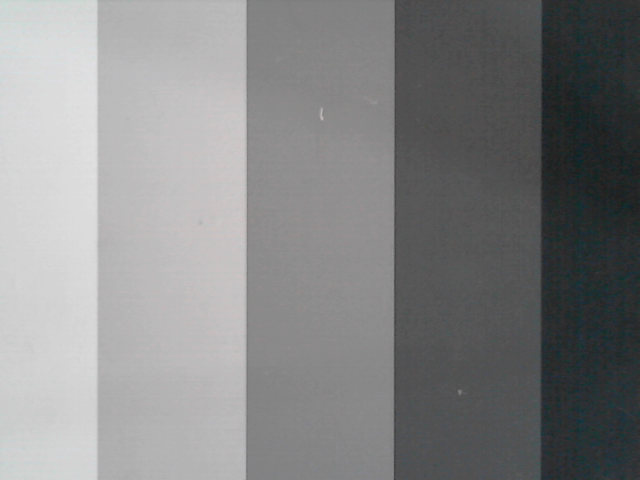
\includegraphics[width=0.7\textwidth]{media/graubild.png}
	\caption{Graukeilbild}
	\label{fig:Graukeilbild}
\end{figure}

\section{Auswertung}
\label{chap:VERSUCH_1_AUSWERTUNG}

Als nächstes müssen wir das Bild wieder einlesen und in seine Farbstufen aufteilen. Das einlesen funktioniert hierbei über die Funktion  cv2.imread(BILDNAME), was uns ein Array aus einzelnen Pixelwerten zurückgibt. Um nun die einzelnen Graustufen des Graukeils in einzelne Farben aufzuteilen, nutzen wir das Index Slicing von python. Wir achten hierbei darauf, dass wir nicht die einzelnen Ränder mit in die Bilder nehmen haben wir jeden Abschnitt 90 pixel breit gemacht und so hoch wie das Ursprungsbild.

Für jede Stufe muss jetzt noch der Mittelwert bestimmt werden. Hierzu wenden wir die Funktion np.mean(STUFE) aus dem Numpy Modul auf die jeweilige Stufe an. Dazu berechnen wir ebenfalls die Standartabweichung mithilfe der Funktion np.std(STUFE) Anschließend haben wir die Einzelnen Graustufen abgespeichert. Unterschieden haben wir hier die Fünf Stufen Weiß, Hellgrau, Grau, Dunkelgrau und Schwarz.

\section{Interpretation}
\label{chap:VERSUCH_1_INTERPRETATION}
Wir haben jetzt die Mittelwerte und die Standartabweichungen berechnet um diese nach der Kalibrierung des Sensors als Vergleich heranziehen zu können.
\end{document}